\documentclass{article}

\usepackage{hyperref}
\hypersetup{
	colorlinks=true,
	linkcolor=blue,
	urlcolor=cyan,}
\usepackage{booktabs}
\usepackage{textgreek}

%%%%%%%%%%%%%%%%%%%%%%%%%%%%%%%%%%%%%%%%%
% Lachaise Assignment
% Structure Specification File
% Version 1.0 (26/6/2018)
%
% This template originates from:
% http://www.LaTeXTemplates.com
%
% Authors:
% Marion Lachaise & François Févotte
% Vel (vel@LaTeXTemplates.com)
%
% License:
% CC BY-NC-SA 3.0 (http://creativecommons.org/licenses/by-nc-sa/3.0/)
% 
%%%%%%%%%%%%%%%%%%%%%%%%%%%%%%%%%%%%%%%%%

%----------------------------------------------------------------------------------------
%	PACKAGES AND OTHER DOCUMENT CONFIGURATIONS
%----------------------------------------------------------------------------------------

\usepackage{amsmath,amsfonts,stmaryrd,amssymb} % Math packages

\usepackage{enumerate} % Custom item numbers for enumerations

\usepackage[ruled]{algorithm2e} % Algorithms

\usepackage[framemethod=tikz]{mdframed} % Allows defining custom boxed/framed environments

\usepackage{listings} % File listings, with syntax highlighting
\lstset{
	basicstyle=\ttfamily, % Typeset listings in monospace font
}

%----------------------------------------------------------------------------------------
%	DOCUMENT MARGINS
%----------------------------------------------------------------------------------------

\usepackage{geometry} % Required for adjusting page dimensions and margins

\geometry{
	paper=a4paper, % Paper size, change to letterpaper for US letter size
	top=2.5cm, % Top margin
	bottom=3cm, % Bottom margin
	left=2.5cm, % Left margin
	right=2.5cm, % Right margin
	headheight=14pt, % Header height
	footskip=1.5cm, % Space from the bottom margin to the baseline of the footer
	headsep=1.2cm, % Space from the top margin to the baseline of the header
	%showframe, % Uncomment to show how the type block is set on the page
}

%----------------------------------------------------------------------------------------
%	FONTS
%----------------------------------------------------------------------------------------

\usepackage[utf8]{inputenc} % Required for inputting international characters
\usepackage[T1]{fontenc} % Output font encoding for international characters

\usepackage{XCharter} % Use the XCharter fonts

%----------------------------------------------------------------------------------------
%	COMMAND LINE ENVIRONMENT
%----------------------------------------------------------------------------------------

% Usage:
% \begin{commandline}
%	\begin{verbatim}
%		$ ls
%		
%		Applications	Desktop	...
%	\end{verbatim}
% \end{commandline}

\mdfdefinestyle{commandline}{
	leftmargin=10pt,
	rightmargin=10pt,
	innerleftmargin=15pt,
	middlelinecolor=black!50!white,
	middlelinewidth=2pt,
	frametitlerule=false,
	backgroundcolor=black!5!white,
	frametitle={Command Line},
	frametitlefont={\normalfont\sffamily\color{white}\hspace{-1em}},
	frametitlebackgroundcolor=black!50!white,
	nobreak,
}

% Define a custom environment for command-line snapshots
\newenvironment{commandline}{
	\medskip
	\begin{mdframed}[style=commandline]
}{
	\end{mdframed}
	\medskip
}

%----------------------------------------------------------------------------------------
%	FILE CONTENTS ENVIRONMENT
%----------------------------------------------------------------------------------------

% Usage:
% \begin{file}[optional filename, defaults to "File"]
%	File contents, for example, with a listings environment
% \end{file}

\mdfdefinestyle{file}{
	innertopmargin=1.6\baselineskip,
	innerbottommargin=0.8\baselineskip,
	topline=false, bottomline=false,
	leftline=false, rightline=false,
	leftmargin=2cm,
	rightmargin=2cm,
	singleextra={%
		\draw[fill=black!10!white](P)++(0,-1.2em)rectangle(P-|O);
		\node[anchor=north west]
		at(P-|O){\ttfamily\mdfilename};
		%
		\def\l{3em}
		\draw(O-|P)++(-\l,0)--++(\l,\l)--(P)--(P-|O)--(O)--cycle;
		\draw(O-|P)++(-\l,0)--++(0,\l)--++(\l,0);
	},
	nobreak,
}

% Define a custom environment for file contents
\newenvironment{file}[1][File]{ % Set the default filename to "File"
	\medskip
	\newcommand{\mdfilename}{#1}
	\begin{mdframed}[style=file]
}{
	\end{mdframed}
	\medskip
}

%----------------------------------------------------------------------------------------
%	NUMBERED QUESTIONS ENVIRONMENT
%----------------------------------------------------------------------------------------

% Usage:
% \begin{question}[optional title]
%	Question contents
% \end{question}

\mdfdefinestyle{question}{
	innertopmargin=1.2\baselineskip,
	innerbottommargin=0.8\baselineskip,
	roundcorner=5pt,
	nobreak,
	singleextra={%
		\draw(P-|O)node[xshift=1em,anchor=west,fill=white,draw,rounded corners=5pt]{%
		Question \theQuestion\questionTitle};
	},
}

\newcounter{Question} % Stores the current question number that gets iterated with each new question

% Define a custom environment for numbered questions
\newenvironment{question}[1][\unskip]{
	\bigskip
	\stepcounter{Question}
	\newcommand{\questionTitle}{~#1}
	\begin{mdframed}[style=question]
}{
	\end{mdframed}
	\medskip
}

%----------------------------------------------------------------------------------------
%	WARNING TEXT ENVIRONMENT
%----------------------------------------------------------------------------------------

% Usage:
% \begin{warn}[optional title, defaults to "Warning:"]
%	Contents
% \end{warn}

\mdfdefinestyle{warning}{
	topline=false, bottomline=false,
	leftline=false, rightline=false,
	nobreak,
	singleextra={%
		\draw(P-|O)++(-0.5em,0)node(tmp1){};
		\draw(P-|O)++(0.5em,0)node(tmp2){};
		\fill[black,rotate around={45:(P-|O)}](tmp1)rectangle(tmp2);
		\node at(P-|O){\color{white}\scriptsize\bf !};
		\draw[very thick](P-|O)++(0,-1em)--(O);%--(O-|P);
	}
}

% Define a custom environment for warning text
\newenvironment{warn}[1][Warning:]{ % Set the default warning to "Warning:"
	\medskip
	\begin{mdframed}[style=warning]
		\noindent{\textbf{#1}}
}{
	\end{mdframed}
}

%----------------------------------------------------------------------------------------
%	INFORMATION ENVIRONMENT
%----------------------------------------------------------------------------------------

% Usage:
% \begin{info}[optional title, defaults to "Info:"]
% 	contents
% 	\end{info}

\mdfdefinestyle{info}{%
	topline=false, bottomline=false,
	leftline=false, rightline=false,
	nobreak,
	singleextra={%
		\fill[black](P-|O)circle[radius=0.4em];
		\node at(P-|O){\color{white}\scriptsize\bf i};
		\draw[very thick](P-|O)++(0,-0.8em)--(O);%--(O-|P);
	}
}

% Define a custom environment for information
\newenvironment{info}[1][Info:]{ % Set the default title to "Info:"
	\medskip
	\begin{mdframed}[style=info]
		\noindent{\textbf{#1}}
}{
	\end{mdframed}
}
 % Include the file specifying the document structure and custom commands

%----------------------------------------------------------------------------------------
%	ASSIGNMENT INFORMATION
%----------------------------------------------------------------------------------------

\title{Week 5: Electrocardiography (ECG) II}
\author{BIOE 320 Systems Physiology Laboratory} 
\date{}
%----------------------------------------------------------------------------------------

\begin{document}
\large
\maketitle

\section*{Objectives}
\begin{enumerate}
	\item To record ECG measurements from leads I and III in the following conditions: lying down, sitting up, and breathing deeply while sitting.
	\item To use Einthoven's Law to estimate the mean electrical axis and magnitude of the QRS complex.
\end{enumerate}

\section*{Background}


\subsection*{Electrical Activity of the Heart (Review)}
\begin{figure}[h]
\centering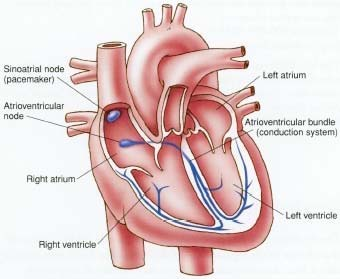
\includegraphics[width=0.4\textwidth]{../images/ECG_II_1a.jpg}
\centering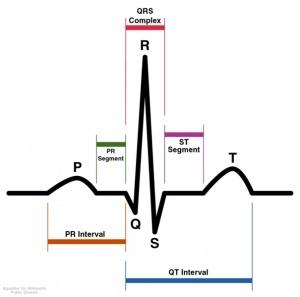
\includegraphics[width=0.3\textwidth]{../images/ECG_II_1b.jpg}
\caption{The pacemaker system and the PQRST wave}
\label{pacemaker}
\end{figure}

The heart's electrical system begins at the sinoatrial (SA) node, the primary pacemaker of the heart, where electric potential originates. The polarization spreads throughout the atria, initiating contraction of atrial myocardium (P wave of ECG). The signal then travels to the AV node where it is delayed, allowing time for the blood to leave the atria before ventricular contraction begins. After the AV nodes, the signal is conducted down the left and right bundle branches and the Purkinje fibers to the ventricular myocardium. Depolarization of the ventricles is recorded as the QRS complex in the ECG, and repolarization of the ventricles is recorded as the T wave. This process is summarized in Fig. \ref{pacemaker}. In the last lab, we saw how the heart's electrical activity can be analyzed using an ECG (specifically, the standard bipolar lead II). This week, we will explore how to interpret the magnitude and direction of the ECG signal and how to estimate the mean electrical axis of the QRS complex.

\subsection*{Einthoven's Law}
ECGs are produced by a system of leads attached to the body. One common lead system uses the three standard bipolar limb leads. The electrode placement defines the recorded direction of the lead, when going from the negative to the positive electrode. The ECG is read as the computed difference (magnitude) between the positive and negative electrodes as a change in voltage over time.\\

The standard bipolar lim leads, their polarity, and axes are as follows:
\begin{table}[h]
	\centering
	\begin{tabular}[h!]{ccc}
	\toprule
	Lead & Polarity & Lead Axis\\
	\midrule
	Lead I & right arm (-) to left arm (+) & 180\textdegree\ to 0\textdegree\\
	 Lead II & right arm (-) to left leg (+) & -120\textdegree\ to 60\textdegree\\
	 Lead III & left arm (-) to left leg (+) & -60\textdegree\ to 120\textdegree\\
	\bottomrule
	\end{tabular}
	\end{table}

The placement of the leads is the result of the extension of Einthoven's Triangle, a triangle of three leads that surrounds the heart. The ECG for each lead displays the amplitude of the voltage as projected onto that lead. To determine the value closest to the actual direction of the heart, Lead II is usually used. However, because the three leads are connected in a loop, Kirchoff's Voltage Law (KVL) states that the voltage drop around the loop must be equal to zero, and therefore, Einthoven's Law can be used to determine the value of one lead if we know the value of the other two.

\subsection*{Mean Electrical Axis: Direction}
During the cardiac cycle, the current spreads along specialized pathways, depolarizing the heart in a specific sequence. Consequently, the electrical activity has .directionality, that is, a spatial orientation represented by an electrical axis. The summation of all the vectors occurring in a cardiac cycle (i.e. the preponderant direction of current flow during the cardiac cycle) is called the mean electrical axis (Fig. \ref{axis})

\begin{figure}[h]
\centering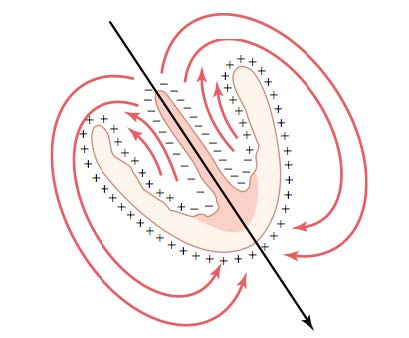
\includegraphics[width=0.5\textwidth]{../images/ECG_II_2.jpg}
\caption{Mean vector through partially depolarized ventricles}
\label{axis}
\end{figure}

Since the QRS complex caused by ventricular depolarization represents the majority of the electrical activity of the heart, you can approximate the mean electrical axis by looking only in this interval. Typically, in an adult, the mean electrical axis lies along a line extending from the base of the apex of the heart and to the left of the interventricular septum pointing toward the lower left rib cage.

\subsection*{Mean Electrical Axis: Magnitude}
The magnitude of the recorded voltage in the ECG is directly proportional to the amount of tissue being depolarized. Most of the mass of the heart is made up of ventricular myocardium. Therefore, the largest recorded waveform, the QRS complex, reflects the depolarization of the ventricles. Furthermore, since left ventricular mass is significantly greater than right ventricular mass, more of the QRS complex reflects the depolarization of the left ventricle and thus the orientation of the mean electrical axis is to the left of the interventricular septum.

\subsection*{ECG Interpretation}
A good mathematical tool for representing the measurement of a lead is the vector. At any given moment during the cardiac cycle, a vector may represent the net electrical activity seen by a lead (Fig. \ref{vector}). The length of the arrow represents the magnitude of the electrical current. The orientation of the arrow represents the direction of current flow. The tip of the arrow represents the positive pole of the electrical current, and the tail represents the negative pole.

\begin{figure}[h]
\centering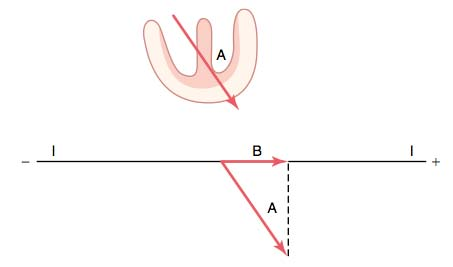
\includegraphics[width=0.7\textwidth]{../images/ECG_II_3.jpg}
\caption{Projection of the mean electrical axis onto lead I (vector B)}
\label{vector}
\end{figure}


\section*{Required Supplies}
\begin{itemize}
	\item BIOPAC student labs lesson L05: ECG I
	\item BIOPAC MP3X data acquisition unit
	\item BIOPAC electrode lead set
	\item BIOPAC disposable vinyl electrodes
	\item Optional but useful: alcohol wipes, abrasive pads, physiology tape, electrode gel
\end{itemize}

\section*{Setting Up}
\begin{enumerate}
	\item Turn on the MP3X acquisition unit by flipping the switch found on the back panel.
	\item Place electrodes and leads on the subject as follows (Fig. \ref{ecg}):\begin{itemize}
		\item Positive (red): inside of left ankle, just above the ankle bone
		\item Negative (white): inside of the right wrist
		\item Ground (black): right ankle bone
	\end{itemize}
	\begin{figure}[h]
	\centering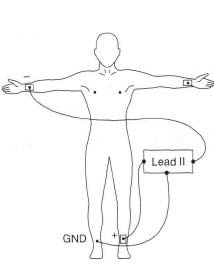
\includegraphics[width=0.4\textwidth]{../images/ECG_I_3.jpg}
	\caption{Schematic of electrode lead placement}
	\label{ecg}
	\end{figure}
	
	\item Plug the electrode cord, SS2L, into channel 2 and connect to the electrodes.
	\item Open Biopac Pro v3.7 (\textbf{not the student lessons})
	\item Go under the MP3X pull-down menu and select Set-up Acquistion (Fig. \ref{setup}).
	\begin{figure}[h]
	\centering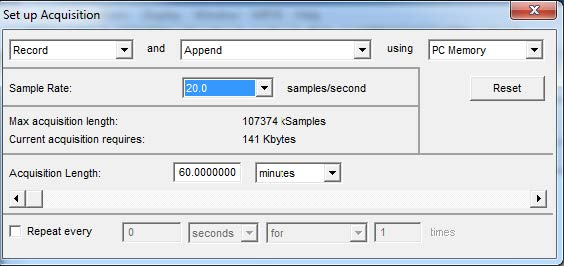
\includegraphics[width=0.6\textwidth]{../images/ECG_I_4.jpg}
	\caption{Set-up acquisition window}
	\label{setup}
	\end{figure}
	
	\item Set the sampling rate to 20/sec. Click reset and close the box.
	\item Go under the MP3X pull-down menu and select Set-up Channels (Fig. \ref{setup_2}).
	\begin{figure}[h]
	\centering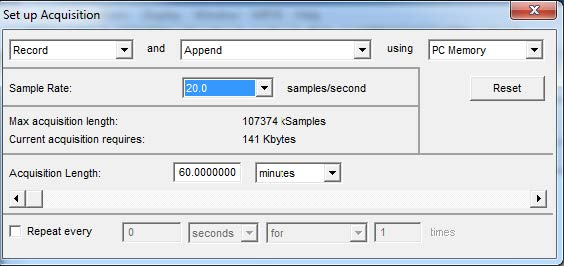
\includegraphics[width=0.6\textwidth]{../images/ECG_I_4.jpg}
	\caption{Set-up channels}
	\label{setup_2}
	\end{figure}
	
	\item Under the presets drop-down arrow, select ECG 0.05 Hz - 150 Hz for both channels 1 and 3.
	\item Check all 3 boxes for channel 2. Deselect all boxes for channels 1 and 3.
	\item Take a sample 30 sec ECG recording by pressing Start.
\end{enumerate}

\subsection*{Changing Sampling Rate}
\begin{enumerate}
	\item Go under the MP3X pull-down menu and select Set-Up Acquisition (Fig. \ref{setup}).
	\item Set the sampling rate to 200/sec.
	\item Take another 30 sec ECG recording by pressing Start.
	\item Close BIOPAC Pro Software. Do NOT remove electrodes or leads from the subject.
	\item What are the differences between the recordings at 20 Hz and 200 Hz?
	\item What criteria should be used to establish an appropriate sampling rate?
\end{enumerate}

\section*{Experiments}
\subsection*{Setting Up}
\begin{enumerate}
	\item Plug the electrode cord into channel 1 and connect the electrodes.
	\item Launch the BIOPAC software by clicking on the BSL Lessons 3.7.6 icon and select L05-ECG-1 as shown in Fig. \ref{lesson}.
		
		\begin{figure}[h]
	\centering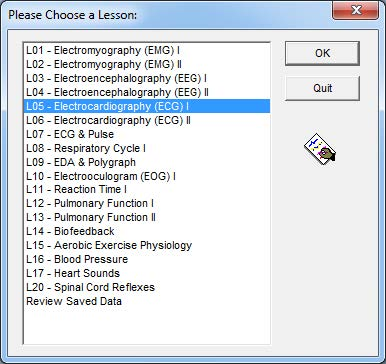
\includegraphics[width=0.6\textwidth]{../images/ECG_I_6.jpg}
		\caption{Selecting BIOPAC lesson L05-ECG-I}
		\label{lesson}
		\end{figure}
\end{enumerate}

\subsection*{Calibration}
\begin{info}
	The calibration procedure establishes the hardware's internal parameters (such as gain, offset, and scaling) and is critical for optimum performance. Pay close attention to the calibration procedure.
\end{info}
\begin{enumerate}
	\item Check that electrodes are still adhered to the skin, If they are being pulled up, you will not get a good ECG signal. The subject must be relaxed and as still as possible during the calibration procedure. The ECG is very sensitive to small changes in voltage caused by contraction of skeletal muscles, so the subject's arms and legs need to be relaxed so that the muscle (EMG) signal does not corrupt the ECG signal.
	\item Click on Calibrate. The calibration procedure will begin and then stop automatically after 8 seconds. At the end of the calibration recording, the screen should resemble Fig. \ref{calibration} below. There should be a regular, periodic ECG waveform with a relatively flat baseline. Some tips for obtaining optimal data:\begin{itemize}
		\item The subject should not talk or laugh during any of the recording segments.
		\item The subject should be in a relaxed state for each recording segment and in the position noted for each segment.
		\item When the subject is asked to sit up, they should do so in a chair, with arms relaxed.
		\end{itemize}
		
		\begin{figure}[h]
	\centering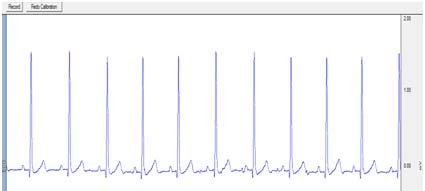
\includegraphics[width=0.6\textwidth]{../images/ECG_I_7a.jpg}
	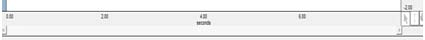
\includegraphics[width=0.6\textwidth]{../images/ECG_I_7b.jpg}
		\caption{Example calibration}
		\label{calibration}
		\end{figure}
		
	\item If the data recording shows any jitter or large baseline drifts, you should redo the calibration by clicking on the Redo Calibration button.
\end{enumerate}

\subsection*{Segment 1: Supine (Laying Down)}
\begin{enumerate}
	\item Prepare for the recording by having the subject lie down and relax with their eyes closed.
	\item Click on Record, and record data for 20 seconds, then click on Suspend at the 20 second mark. Proceed unless:
		\begin{itemize}
			\item The suspend button was pressed prematurely.
			\item An electrode peeled up, causing a large baseline drift, spike, or loss of signal.
			\item The subject has too much muscle (EMG) artifact.
		\end{itemize}
\end{enumerate}

\subsection*{Segment 2: Sitting Up}
\begin{enumerate}
	\item Starting from the supine position, have the subject sit up quickly. Click on Resume and record for another 20 seconds. The recording will continue from the point where it last stopped and a marker labeled "sitting up" will automatically come up when Resume is pressed.\begin{info}
In order to capture the heart rate variation, it is important that you click on Resume to continue recording as quickly as possible after the subject sits up. However, it is also important that you do not click on Resume while the subject is \textit{in the process of} sitting up or you will capture motion artifact.	
\end{info}

	\item Click on Suspend at the end of the 20 second recording segment (at the 40 second mark total). Proceed unless you see any of the conditions described in Segment 1.
\end{enumerate}

\subsection*{Segment 3: Deep Breaths}
\begin{enumerate}
	\item Click on Resume. The recording will continue from the point where it last stopped, and a marker labeled "5 deep breaths" will automatically come up when Resume is pressed.
	\item Record for 20 seconds and have the subject take in 5 deep breaths during recording. The 5 deep breathing cycles should be deeper and slower than normal breathing at rest and should follow one another.
	\item During this time, the person operating the software should insert a marker at the beginning of an inhale and insert another marker at the corresponding exhale. The recorder should label these markers "inhale" and "exhale" (note: the hotkey for a marker is F9).
	\item At the end of the 20 second recording segment, click on Suspend. Note that deep breathing may produce a baseline drift. This is normal and does not necessitate redoing the recording.
\end{enumerate}

\subsection*{Segment 4: Light Exercise}
\begin{enumerate}
	\item Disconnect the electrode leads (do not remove the electrodes) and have the subject move to a safe area and perform an exercise that will elevate their heart rate fairly rapidly (e.g. push-ups, jumping jacks).
	\item Immediately after the exercise, have the subject assume a sitting position and reconnect the electrode leads: \begin{itemize}
		\item Positive (red): inside of left ankle, just above the ankle bone
		\item Negative (white): inside of the right wrist
		\item Ground (black): right ankle bone
	\end{itemize}
	
	\item After the subject is stationary, click on Resume. The recording will continue from the point where it last stopped, and a marker labeled "after exercise" will automatically come up when you click Resume.
	\item Record the post-exercise ECG for 60 seconds, then click on Suspend (120 second mark total). Again, the baseline may drift, but this is fairly normal unless iti s excessive.
	\item Click on Done. A pop-up window with six options will appear, select "Analyze Data From Current Subject."
	\item Remove the electrode cable pinch connectors and peel off the electrodes. Throw out the electrodes. The electrodes may leave a slight ring on the skin for a few hours, which is quite normal.
\end{enumerate}

\section*{Data Analysis}
\subsection*{Segment 1}
\begin{enumerate}
	\item Determine the time and beats per minute of three cardiac cycles and record in Table 1 of the handout. Calculate the means.
	\item Complete Table 2 for the different components of the ECG for Cardiac Cycle 1.
	\item Is there always one P wave for every QRS complex? If not, what would this signify?
	\item Compare and contrast the shape (duration and amplitude) of the P and T waves. Give the mechanical and electrical reasons for the differences.
\end{enumerate}

\subsection*{Segment 2}
\begin{enumerate}
	\item Complete Table 3.
	\item Explain the observed heart rate variations in sitting up vs. supine positioning. Describe the physiological mechanisms causing these differences.
\end{enumerate}

\subsection*{Segment 3}
\begin{enumerate}
	\item Complete Table 4.
	\item Are there differences in the cardiac cycle with the respiratory cycle (inspiration vs. expiration)? If so, what is the physiological basis for these differences?
\end{enumerate}

\subsection*{Segment 4}
\begin{enumerate}
	\item Complete Tables 5 and 6.
	\item What changes occurred in the duration of systole and diastole between resting and immediately after exercise? What could account for these changes?
\end{enumerate}

\begin{warn}
	The data that you will need for your post-lab is located on (find a good location).
\end{warn}
\end{document}
